
\documentclass[aps,prl,reprint]{revtex4-2}
\usepackage{gensymb}
\usepackage{wrapfig}
\usepackage{graphicx}
\usepackage{amsmath}
\usepackage{hyperref}
\usepackage{dsfont}
\usepackage{relsize}
\usepackage{wrapfig}
\usepackage{graphicx}
\usepackage{hyperref}
\hypersetup{colorlinks=true, citecolor=blue, urlcolor=blue, linkcolor=blue}


\begin{document}

% Use the \preprint command to place your local institutional report
% number in the upper righthand corner of the title page in preprint mode.
% Multiple \preprint commands are allowed.
% Use the 'preprintnumbers' class option to override journal defaults
% to display numbers if necessary
%\preprint{}

%Title of paper
\title{Hall Effect Lab}

% repeat the \author .. \affiliation  etc. as needed
% \email, \thanks, \homepage, \altaffiliation all apply to the current
% author. Explanatory text should go in the []'s, actual e-mail
% address or url should go in the {}'s for \email and \homepage.
% Please use the appropriate macro foreach each type of information

% \affiliation command applies to all authors since the last
% \affiliation command. The \affiliation command should follow the
% other information
% \affiliation can be followed by \email, \homepage, \thanks as well.
\author{Trevor Smith, Alex Storrer}
\email[]{smith.tr@northeastern.edu}
\homepage[]{https://github.com/trevorm4x/}
%\thanks{}
%\altaffiliation{}
\affiliation{Northeastern University}


\date{\today}

\begin{abstract}
	A sample semiconductor wafer was analyzed to determine its intrinsic properties. 
	Using two different methods, it was determined that the semiconductor was a p-type.
	Its resistivity $\rho$ was measured at $9\ \pm\ 2\ \Omega\ cm$, higher than the accepted
	range of 5.86-6.31 $\Omega\ cm$. The carrier mobility of the semiconductor was  
	measured at 320 \pm 60 cm/V$\cdot$s, close to the accepted value of 455 cm/V$\cdot$s. The 
	carrier concentration was measured at 2.26 \times 10$^{15}$ \pm 9 \times 10$^{13}$  
	holes per cm$^{3}$, which is within the range of $10^{14}-10^{20}\ cm^{-1}$. Given
	the difficulty of measuring $\rho$ accurately with this test procedure and the
	interconnectedness of these values, where carrier concentration determines accepted
	carrier mobility ranges, these numbers are very reasonable.
\end{abstract}


\maketitle

% body of paper here - Use proper section commands
% References should be done using the \cite, \ref, and \label commands
\section{Introduction}
Semiconductors are an incredibly important technology with a wide variety of applications, 
including solar cells, light-emitting diodes (LEDs), and computers. One element of their 
importance is due to their behavior as a conductor - as they heat up their conductance 
\emph{increases} as opposed to regular metals. Their usefulness and application is closely 
tied to their makeup, with one of the broadest classifications being between their doping causing
them to behave as p-type or n-type semiconductors. \\

In this lab we will probe the behavior of a semiconductor using various methods, quickly
finding that conventional methods for measuring resistance are not sufficient here, due especially
to a semiconductor's non-ohmic nature. This motivates the need for more precise measurements,
especially the 4-wire method which will be explored in more detail later. We will also heat the
semiconductor on one side to produce a voltage by which we can determine the major carrier type, 
p or n. Lastly, we will use the Hall Effect, where a charge traveling in a magnetic field 
will be pushed in a direction orthagonal to both its movement and the field, to determine the
charge carrier type again, the carrier density, and finally the carrier mobility. 

\section{Apparatus}

The apparatus consisted of the following.

\begin{itemize}
	\item Doped silicon wafer
	\item Pre-Wired circuit board
	\item Carbide scriper
	\item 2 Soldering irons, indium solder, lead-tin solder
	\item Rubber cement
	\item DC Power Supply, GPS-3030DD
	\item 2 Digital Multimeters, GW8145
	\item Electromagnet, GMW3470
	\item LaTeX, document preparation software
	\item Jupyter Notebook
	\item Python compiler
\end{itemize}

\section{Make Hall Sample}

\subsection{Procedure}

\begin{wrapfigure}{o}{.28\textwidth}
	\begin{center}
		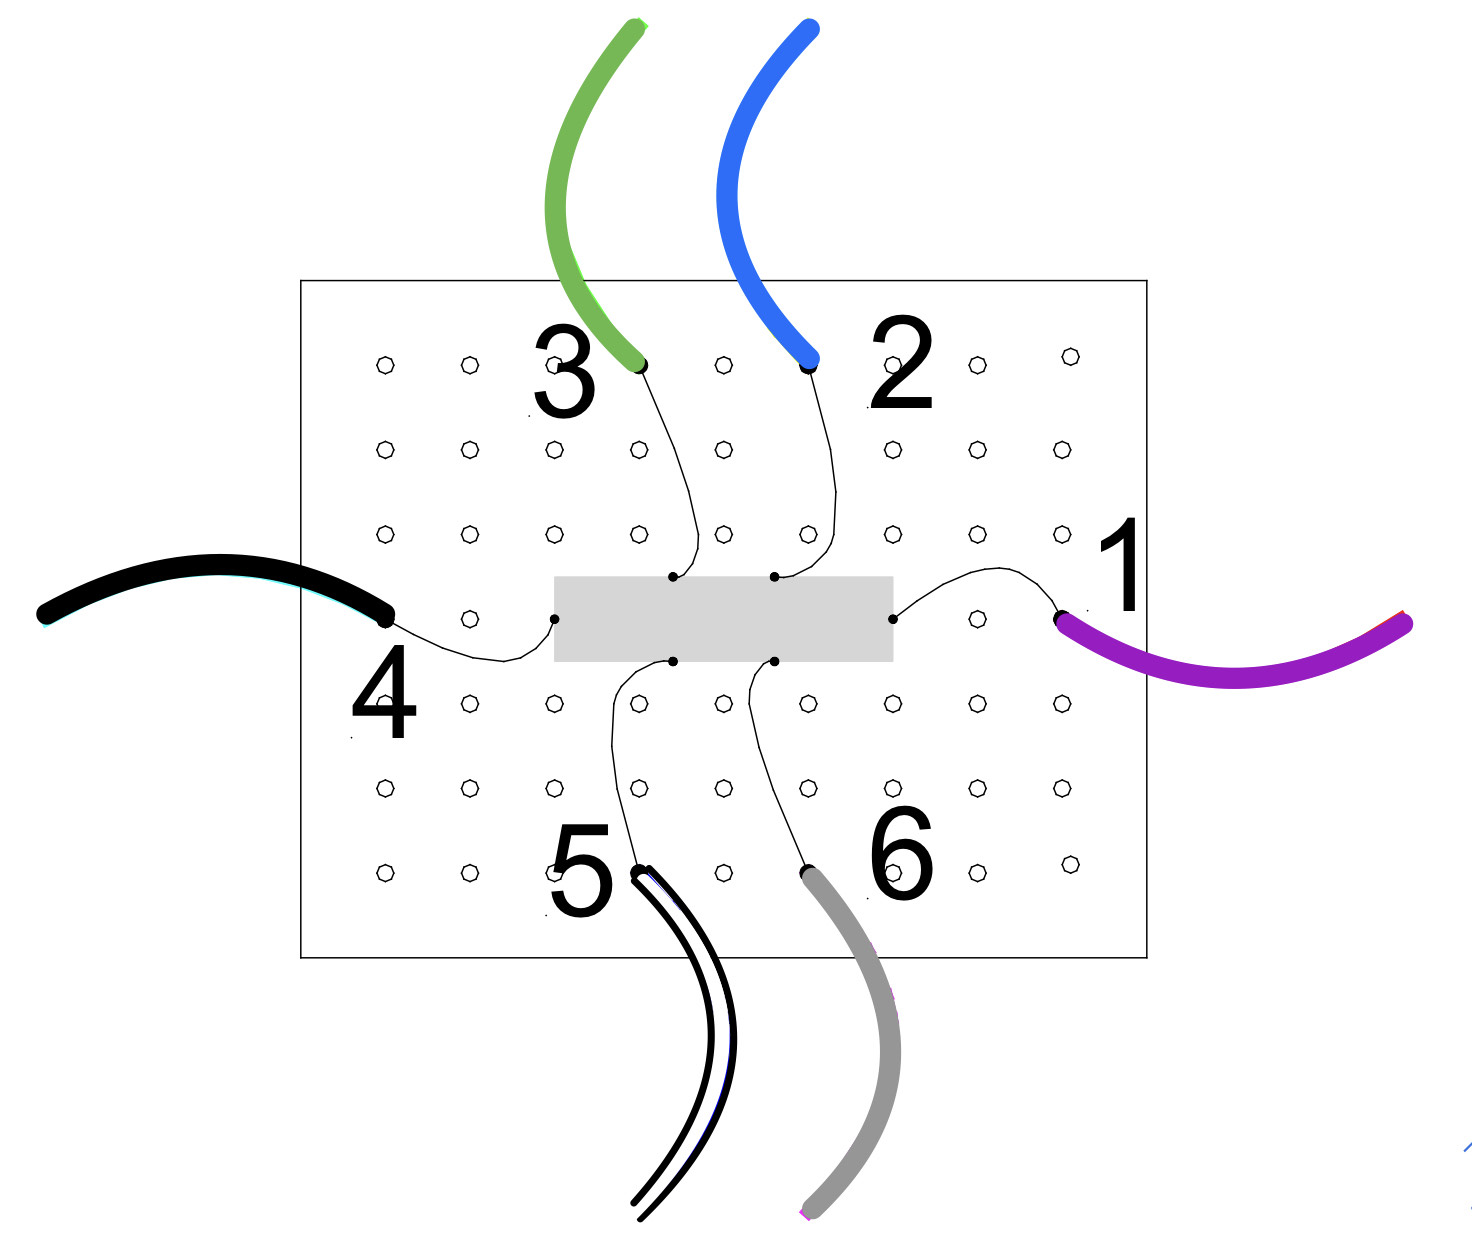
\includegraphics[width=0.29\textwidth]{../Images/l2_WireDiagram.jpg}
	\end{center}
	\caption{\label{colors} Coloring/numbering convention of the experimental setup.}
\end{wrapfigure}

The first step of the experiment was to prepare a hall sample. This involved selecting
and measuring a Si wafer, securing it to a circuit board prefitted with six insulated wires,
and securing the wires to the four sides of the sample with thin wire and indium solder. 
Before soldering, the wafer was measured, width, height, and thickness. 
The configuration of the wires connected to the semiconductor is shown in \ref{colors}. \\

Resistances between each pair of wires was measured with an Ohmeter. One wire was found to have
a bad solder and was resoldered until all measured resistances were $< 1\ M\Omega$. \\

Ohmic behavior was tested by generating a R(V) and I(V) curve. A current was applied to 
the two end wires and varied, such that the resulting power was between -0.1 and 0.1 Watts. \\

\subsection{Results and Conclusion}

Results for the two-wire method of measuring resistance are shown below, where in order to 
measure resistance between two nodes a ohmmeter is simply connected between them. This method
is known to be inaccurate and a more precise method is used later in the experiment, however
this verifies the test setup is correct.

\begin{table}[h]
\begin{tabular}{lr}
\toprule
Wire Pair &  Resistance ($\Omega$) \\
\midrule
\hline
3-2       &     22760.0 \\
3-6       &     24550.0 \\
3-5       &     66430.0 \\
3-4       &     26940.0 \\
3-1       &     28570.0 \\
2-6       &     11213.0 \\
2-5       &     12445.0 \\
2-4       &     12060.0 \\
2-1       &     11665.0 \\
6-5       &     51390.0 \\
6-4       &      8893.6 \\
6-1       &      9566.0 \\
5-4       &    171760.0 \\
5-1       &    176260.0 \\
4-1       &     12296.0 \\
\hline
\hline
\bottomrule
\end{tabular}
\caption{\label{pairs}Resistance for each combination of wires,\\ given by their numbering convention matching that in \ref{colors}.}
\end{table}

Next we probed the behavior of the semiconductor as a resistor, measuring voltage and current as
a voltage was applied, starting at 0 and increasing until the power was just under 0.1 Watts. 

% WHY DOES RESISTANCE

\begin{figure}[h]
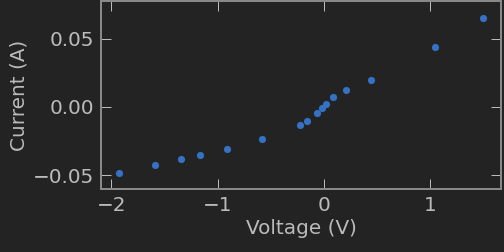
\includegraphics[width=0.5\textwidth]{../Images/l2_a_1.png}
\caption{\label{figA}I(V) shows different behavior closer to zero than elsewhere. }

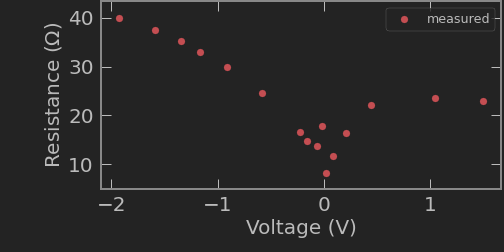
\includegraphics[width=0.5\textwidth]{../Images/l2_a_2.png}
\caption{\label{figA}R(V) is not constant, demonstrating non-ohmic behavior.}
\end{figure}


In this phase of the experiment, we were able to demonstrate that the test setup had no 
major issues and that the behavior of the semiconductor is non-ohmic. This is likely due
to a certain voltage threshold inherent to semiconductors where resistance increases as 
the threshold is approached. If more voltages were able to be tested, we would see a decreasing
trend with increasing voltage after this initial peak.\\

\newpage

\section{The 4-Wire Method for Measuring Resistivity of a Doped Silicon Wafer}

\subsection{Procedure}

\begin{wrapfigure}{o}{.25\textwidth}
	\begin{center}
		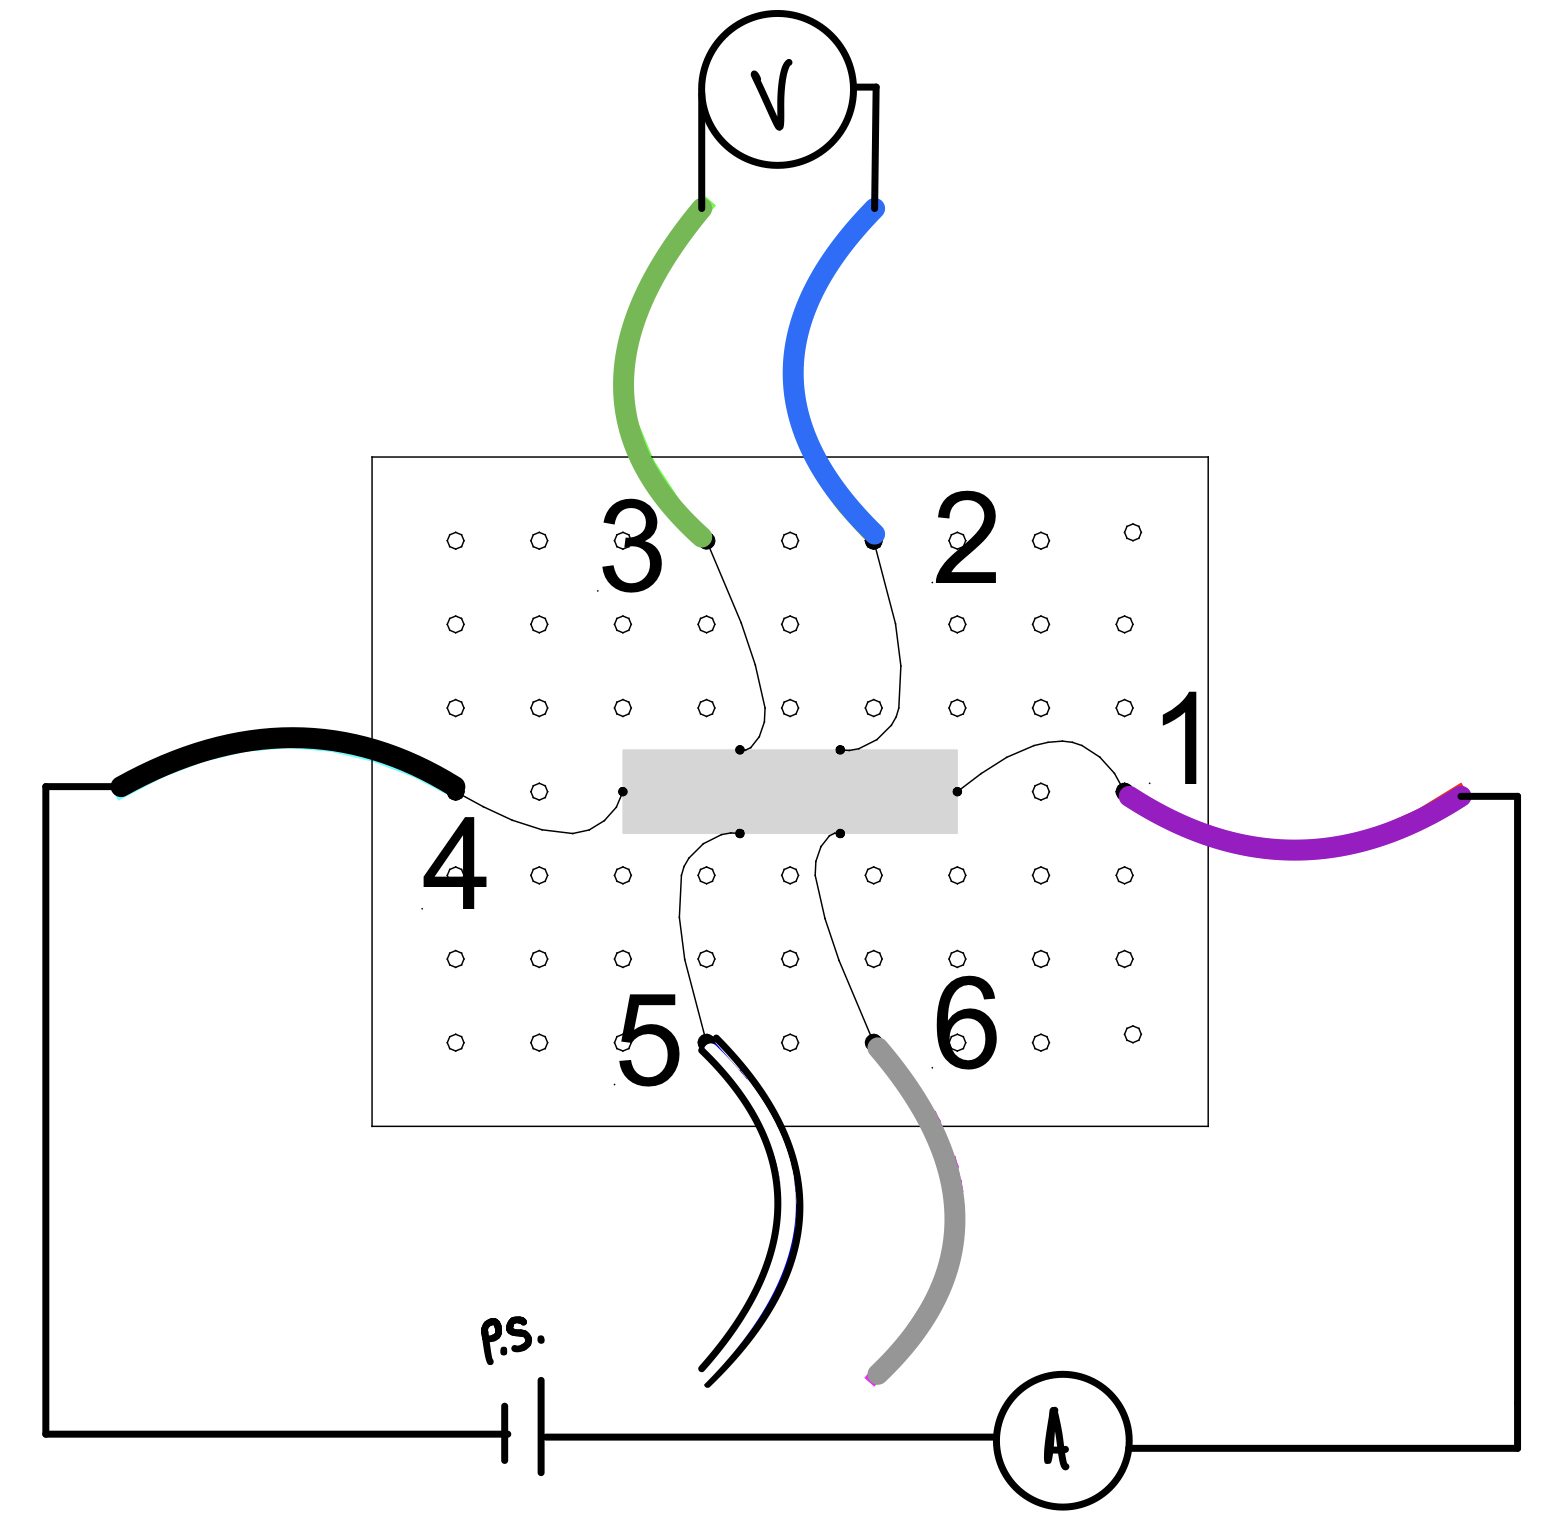
\includegraphics[width=0.29\textwidth]{../Images/l2_4Wire.jpg}
	\end{center}
	\caption{\label{4wire} Four-Wire measurement configuration.}
\end{wrapfigure}

The 4-wire method was used to more accurately measure the resistivity of our material. In this
method, instead of attaching an ohmmeter across the two wires, resulting in a resistivity
that includes the wires and connections between said wires, two measurements that are 
orthagonal are performed. An ampmeter is used to measure an applied current across the same
two wires (which gives an accurate measure of current because the circuit is isolated along 
that path), and a voltmeter is used to measure immediately along either side of the resistor,
in this case across wires 2-3 and 5-6, where any resistance does not cause a meaningful 
voltage drop.\\

These values for resistance were then used to calculate the material's resistivity $\rho$,
using the earlier measurements of the wafer's dimensions. \\

Finally, measurements across the side wires were repeated with the ohmmeter for comparison. \\

\subsection{Results and Conclusion}

Two values for $\rho$ were attained using equation \ref{rho}, and a comparison was
made between the two methods for measuring resistance, given in table \ref{rhotable}. 

\begin{equation}
	\mathlarger{\rho=\frac{R\cdot A}{L}}
    \label{rho}
\end{equation}

\begin{table}[h!]
\renewcommand{\arraystretch}{1.45}
\setlength{\tabcolsep}{10pt}
\begin{tabular}{lrrr}
\toprule
Path &  4-Wire R ($\Omega$) &  2-Wire R ($\Omega$) &       $\rho\ (m\Omega)$ \\
\midrule
2-3 &         147 &     20200.0 &  0.079131 \\
5-6 &         235 &    213600.0 &  0.102832 \\
\bottomrule
\end{tabular}
\end{table}
There is indeed a substantial difference between the two measuring methods in this case,
three orders of magnitude. Additionally, the two 4-wire measurements were different by about 2x,
but the 2-wire measurements were different by an order of magnitude. Thus, the relative variance
of the 2-wire method is much higher, implying that it has both worse accuracy and precision.\\

This is of course due mostly to the quality of the solder connections between the wires and the
semiconductor, meaning that the connections on one side were probably just worse than the other 
side.\\

Because two measurements of $\rho$ were calculated, which are both measuring the same property
of the same material, they were taken as a small distribution, with the mean as the measured
value and the uncertainty the standard deviation. Our measured value is therefore
$9\ \pm\ 2\ cm\Omega$.

\section{Thermoelectric Determination of the Carrier Type}

In order to determine the expected carrier concentration, it is necessary to determine wether
the semiconductor is p-type or n-type. This was done by connecting the wires 1-4, on the
shorter ends of the rectangle as seen in \ref{colors}, to a voltmeter and applying heat 
with a sordering iron. To explain why this makes sense in short, heating one end of a 
doped semiconductor will cause charge carriers of the same sign as the type to move away from 
the heated end. \\

To unpack why, we first note that the Fermi energy for a non-doped semiconductor is halfway
between the valence band and the conduction band. At zero kelvin, the probabiliy of finding 
an electron at a certain maximum energy level is a constant.
When the semiconductor is heated, this Fermi energy is not
a constant, but rather shows a widening distribution of electron probabiliy density eventually
dipping into the conduction band and removing a slice from the valence band. 
Now, given the fact that this Fermi energy is much closer to the valence band for p-type 
semiconductors and much closer to the conduction band for n-type semiconductors, we can
piece everything together. After applying heat on one side, for a p-type semiconductor, electrons
are forced out of the valence band creating positive holes, and for an n-type semiconductor
electrons are pushed out into the conduction band. These charge carriers then are able to
diffuse like a gas throughout the semiconductor, producing a current of the semiconductor's type
towards the opposite side. \\

Contact 1 was connected to the negative node of the voltmeter, and contact 4 was connected
to the positive node of the voltmeter. Upon heating the wafer near contact 1, we observed an
increase in the reading on the voltmeter, indicating that a positive current was flowing towards
contact 4. Upon heating the wafer near contact 1, we observed a decrease in the reading on
the voltmeter, indicating that a positive current was flowing towards contact 1 into the negative
node on the voltmeter. From this, with the reasoning above, we concluded that our semiconductor
was a p-type semiconductor. \\


\section{Hall Effect, Carrier Concentration and Mobility}

Finally, we will utilize the Hall Effect to reproduce the previous carrier type conclusion, 
measure the carrier density, and measure the carrier mobility. 

\subsection{Procedure and Results}

\subsubsection{Electromagnet Calibration}

We began by calibrating the electromagnet using a Gaussmeter, measuring magnetic field B as
a function of current and curve fitting the data to obtain $\alpha$ in eq. \ref{alpha}.

\begin{equation}
	\mathlarger{B(I_M) = \alpha I_M}
    \label{alpha}
\end{equation}

\begin{figure}[h]
	\begin{center}
		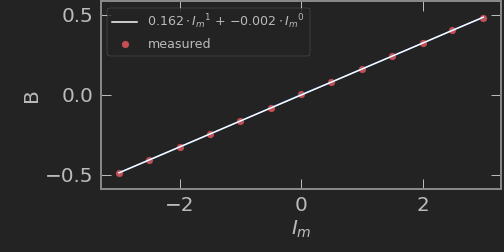
\includegraphics[width=0.48\textwidth]{../Images/l2_d_4.png}
	\end{center}
	\caption{\label{current} Magnetic field with varying current.}
\end{figure}

Where B is electric field in Teslas, $I_m$ is current, and $\alpha$ is a constant relating
the electromagnet's input current to its output magnetic field. This fit value was measured as
0.162 T/A. The precision of this fit is very high and therefore the uncertainty should be
considered irrelevant. However, this value was the second one calculated, as different
behavior was observed on different days, and as such this value may be a source of error even
though the uncertainty is difficult to quantify. \\

\subsubsection{Measure Hall Voltage}

Next, a current was applied from contact 1 to contact 4. 
Then, a voltmeter was connected across the wafer in the 
opposite direction, from contact 2 to contact 6. Finally, this setup was inserted into the
magnetic field produced by the electromagnet, such that the magnetic field was entering into
the top of the wafer, orthagonal to both the voltmeter and the current. The applied current to 
the electromagnet was then varied, with the resulting Hall Voltage recorded at each value. This
resultant voltage is recorded in \ref{V_h_I} with respect to the input current, and in \ref{V_h_B}
with respect to the magnetic field, transformed from current using $\alpha$. \\

\begin{figure}[h]
	\begin{center}
		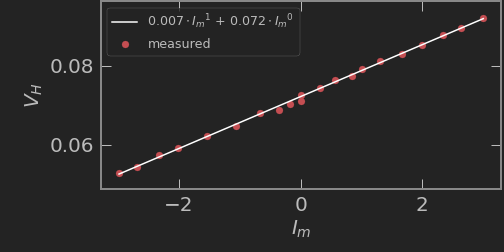
\includegraphics[width=0.48\textwidth]{../Images/l2_d_4a_all.png}
	\end{center}
	\caption{\label{V_h_I} Measured voltage across the semiconductor for all electromagnet 
	input currents. }
\end{figure}

\begin{figure}[h]
	\begin{center}
		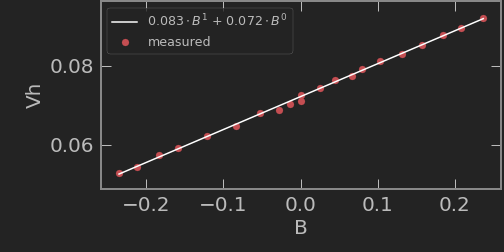
\includegraphics[width=0.48\textwidth]{../Images/l2_d_4b.png}
	\end{center}
	\caption{\label{V_h_B} Measured voltage across the semiconductor for all magnetic fields
		produced. }
\end{figure}

It is important to note that $V_H$ does not cross the origin. It was observed during the
thermoelectric determination of the carrier type that the voltage when no current was applied
was not zero as well. It may be that the voltmeter was simply not calibrated to zero.

\subsubsection{Determine Carrier Type from Hall Voltage}

The Hall Effect can also be used to repeat the determination of carrier type. First, consider the
equation for this effect, given by \ref{hall}.


\begin{equation}
	\mathlarger{F = q (v \times B)}
    \label{hall}
\end{equation}

Interestingly, it is not the direction of the Hall Voltage that informs us the direction of the
force, because the applied current is only in one direction. Either postitive charge carriers are
moving in the same direction as the current, or negative charge carriers are moving in the 
opposite direction of the current, regardless, the resultant force will be in the same 
direction. A determination of carrier type is based on the frequency of a given charge carrier
in the semiconductor - in a p-type there will be more positive charge carriers on the bottom of
the device because there are more postive charge carriers in such a material, with the opposite
being true, resulting in the ability to differentiate semiconductor type from the polarity of the 
voltage. \\

\begin{figure}[h]
	\begin{center}
		\includegraphics[width=0.48\textwidth]{../Images/l2_Magnet.jpg}
	\end{center}
	\caption{\label{magnet} Diagram of applied magnetic field, orientation of silicon wafer,
		current, and voltmeter.}
\end{figure}

In order to conclude the charge carrier type, we must dissect fig. \ref{magnet} and fig. 
\ref{V_h_B}. We can see that with increasing magnetic field, we have an increasing $V_H$. 
By referencing the orientation of the positive node of the voltmeter, which is on top of the
wafer, we find that there is an accumulation of positive charge at the top node. By using the
right-hand-rule, where the index finger is pointed along the current (left and out of page), 
the middle finger is pointed out from the palm and in the direction of magnetic field (towards
right of page), and following the resulting direction of the thumb (for those with conventional
hand configurations), we can see that the Hall Effect will result in a buildup of charge on the 
top node. We can then conclude that positive charge buildup in the direction of the Hall Force
means that we are dealing with a p-type semiconductor with more positive than negative charge 
carriers, which is in agreement with the earlier result.

\subsection{Determine the Carrier Density}

We can use the derived slopes for $\frac{dV_H}{dB}$ to compute the carrier concentration, using
equation \ref{slopes}.

\begin{equation}
	\mathlarger{n=\frac{BI}{V_Hed}} ;\ 
	\mathlarger{n=\frac{dV_H}{dB}^{-1}\frac{I}{ed}}
    \label{slopes}
\end{equation}

Where n is the target value charge carrier concentration, $dV_H/dB$ is the discussed slope, I is
the applied current, e is the fundamental charge, and d is the thickness of the material. \\


\begin{table}[h]
\begin{tabular}{lrr}
\toprule
{} &  Measured Value &  Uncertainty \\
\hline
$dV_H/dB$ (V/T) &        0.040520 &     0.000357 \\
I (A)         &        0.007913 &     0.000026 \\
d (m)         &        0.000540 &     0.000020 \\
\hline
\hline
\bottomrule
\end{tabular}
\caption{The measured values, with uncertainty, used to calculate n.}
\end{table}

The uncertainty of the slope $dV_H/dB$ was taken as the mean absolute error of the fit, which
was quite small due to the fit being quite good. The uncertainty of $I$ was calculated 
considering that this applied current was meant to be constant, and yet varied seemingly randomly
during the experiment, and is taken as the standard deviation. The uncertainty of d is taken
somewhat arbitrarily, considering that the micrometer is very accurate and yet varies depending
on how hard the measurer clamps it. The final calculated value was therefore $2.25e21\ \pm\ 0.09e21\ m^-3$.


\subsection{Determine the Carrier Mobility}

Finally, we can compute the carrier mobility $\mu$ using the above values for $\rho$ and n. 
These values are related in the equation below.


\begin{equation}
	\mathlarger{ \rho = \frac{1}{n\ e\ \mu} ;\ \ \ 
	\mu = \frac{1}{n\ e\ \rho} }
\label{mu}
\end{equation}

The final calculated value was found to be $320 \pm 60$ cm/Vs, three sigma removed from
the accepted value of 455 cm/Vs, with the most significant error stemming from the two discordant
measures of $\rho$.


\section{Summary}
The behavior of a semiconductor was successfully analyzed, including an investigation into its
resistivity, charge carrier type, carrier density, and carrier mobility. \\

Our test setup was found to be adequate, although the significant difference in apparent 
solder quality from contact to contact likely contributed to our measure of $\rho$ later.
In fact, on the third day of the experiment some solders were redone before beginning the
Hall Voltage phase, and in fact overall the equipment was deemed quite difficult to work with.\\

Regardless, we were able to measure a value of $\rho$ which had at least a reasonable correlation
with the expected value. These measurments, due to their significantly varying values, caused
the most significant uncertainty which propogated to our final calculations of $\mu$. These
differences may have been due to solder connections, measurements between the contacts, but was
likely significantly effected by our operating range of 0.1 Watts corresponding to a voltage
below the usual operating voltage of the semiconductor, where it does not exhibit semiconductance
properties as strongly. In fact, the upper range of the absolute value of voltage corresponded
with the highest measured resistances, where if that range of voltages were extended higher we 
would see more typical semiconductor behavior where higher voltages correspond to lower 
resistances. \\

In the heating experiment, we were able to conclude that the semiconductor is of the p-type, 
a result corroborated in the Hall Voltage experiment. \\

The Hall Voltage experiment allowed us to produce a reasonable measurement for $\mu$ and n. 
It is worth clarifying that the value for n is not listed in our final summary table because
there is a very large range of accepted n, and the accepted value of $\mu$ is a function of
n. As mentioned earlier, the uncertainty in $\mu$ was due almost entirely due to the uncertainty
in $\rho$, however it wouldn't make sense to say that that any error in n could lead to error in
$\mu$, due to their tangled relationship where $\mu$ is calculated from n but n determines the
accepted value for $\mu$ as well. Therefore in improving these measurements it may be 
most pertinent to focus on improving $\rho$ accuracy.

\begin{widetext}
\begin{center}
\begin{table}[h]
\renewcommand{\arraystretch}{1.35}
\setlength{\tabcolsep}{10pt}
\caption{\label{rhotable}Measured and accepted values of the speed of light and refractive index of various materials.}
\begin{tabular}{|c|c|c|c|c|}
%\hline
\toprule
Property & Measured Value &  Accepted Value & Refs. &   Deviation \\
\colrule
Resistivity, \rho & $9 \pm\ 2\  \Omega cm$  & 5.86-6.31 $\Omega$cm & \cite{res} & 2 \sigma \\

\colrule
Carrier Density, $n$ & $2.26 \times 10^{15}\ \pm\ 9 \times 10^{13}\ cm^{-3}$ & 1.0 \times 10$^{14}$ - 1.0 \times 10$^{20}$ cm$^{-3}$  & \cite{res} & 0 \sigma \\

\colrule
Carrier Mobility, \mu & $320\ \pm\ 60\ cm/V\cdot s$ & 455 cm/V$\cdot$s & \cite{res} & -3 \sigma \\
%\hline
\botrule
\end{tabular}
\end{table}
\end{center}
\end{widetext}


\begin{thebibliography}{9}
%
\bibitem{res}
University of Colorado, Semiconductor Properties: \\
\href{https://ecee.colorado.edu/~bart/book/mobility.htm}{https://ecee.colorado.edu/~bart/book/mobility.htm}

\end{thebibliography}


\end{document}
%
% ****** End of file apstemplate.tex ******

